\section{资料与方法}

\subsection{研究设计与主要终点}
本研究为回顾性方法学研究，使用既有项目中的患者级数据划分与结果归档重新构建论文叙事。全文以 \textbf{CentralLNM} 作为唯一主要终点，所有主结果均围绕该终点展开；整体淋巴结转移（LNM）与侧方淋巴结转移（LateralLNM）仅在原始临床基线中作为补充信息呈现，不参与主文主线竞争。

\subsection{统一公平比较协议}
为保证不同方法之间的可比性，主文仅保留满足以下条件的结果：
\begin{itemize}[leftmargin=1.8em]
  \item 统一采用患者级 5-fold 交叉验证；
  \item 不同方法尽量共享同一患者划分与主要评价口径；
  \item 主要比较指标为测试集 AUC 的均值$\pm$标准差；
  \item 同步报告 ACC、F1、Sensitivity（Sen）与 Specificity（Spe）；
  \item 对深度学习主模型额外报告逻辑依从率（$P_{central}\le P_{lnm}$）与风险分层表现。
\end{itemize}

\subsection{原始临床基线模型}
原始临床基线直接读取术前临床 Excel 数据，通过图像编号与患者级分组文件对齐，再以患者为单位进行特征聚合和建模。候选变量包括性别、年龄、BMI、超声形态学表现、微钙化、病灶大小、血流信号以及术前超声提示的淋巴结异常等。建模流程遵循临床统计分析的常见顺序：先进行单因素 Logistic 回归筛选，再进入多因素 Logistic 回归，并在测试集报告主要判别指标。该部分的意义在于提供一个不依赖深度特征和预处理 embedding、更加符合临床论文语境的真实术前基线。

\subsection{传统影像组学比较}
传统影像组学部分在相同患者级 5-fold 划分下，仅保留两条路径：ROI Radiomics-only 与 Clinical+ROI Radiomics。影像侧采用传统统计影像特征，患者级聚合后分别输入多种经典机器学习模型。正文展示最佳模型汇总与 ROC 对比，并补充两条 pipeline 的多模型比较表。

\subsection{多模态深度学习融合主模型}
深度学习主模型基于多模态超声输入，核心设计包括三个部分。第一，采用患者级多实例学习（MIL）而非简单片级平均，以更符合临床样本组织形式。第二，使用临床主导的门控融合方式，将临床信息作为稳定主路径，再按需引入影像信息。第三，引入软先验约束损失，惩罚违反 $P_{central}\le P_{lnm}$ 的预测，以强化与临床常识一致的输出结构。

设患者包含 $N$ 个实例，实例编码器输出为 $h_i\in\mathbb{R}^D$。Attention-MIL 的患者级影像表征为：
\begin{equation}
H_{img}=\sum_{i=1}^{N} a_i h_i ,
\end{equation}
其中 $a_i$ 为归一化注意力权重。临床向量编码为 $H_{clin}$ 后，通过门控向量 $G=\sigma(W H_{clin}+b)$ 控制影像信息注入，最终融合表示为：
\begin{equation}
H_{final}=H_{clin}+G\odot H_{img}.
\end{equation}
为了维持双任务输出的临床一致性，训练时加入软约束：
\begin{equation}
L=L_{cls}+\alpha \cdot \mathrm{mean}\,\max(0, P_{central}-P_{lnm}).
\end{equation}

\begin{figure}[H]
\centering
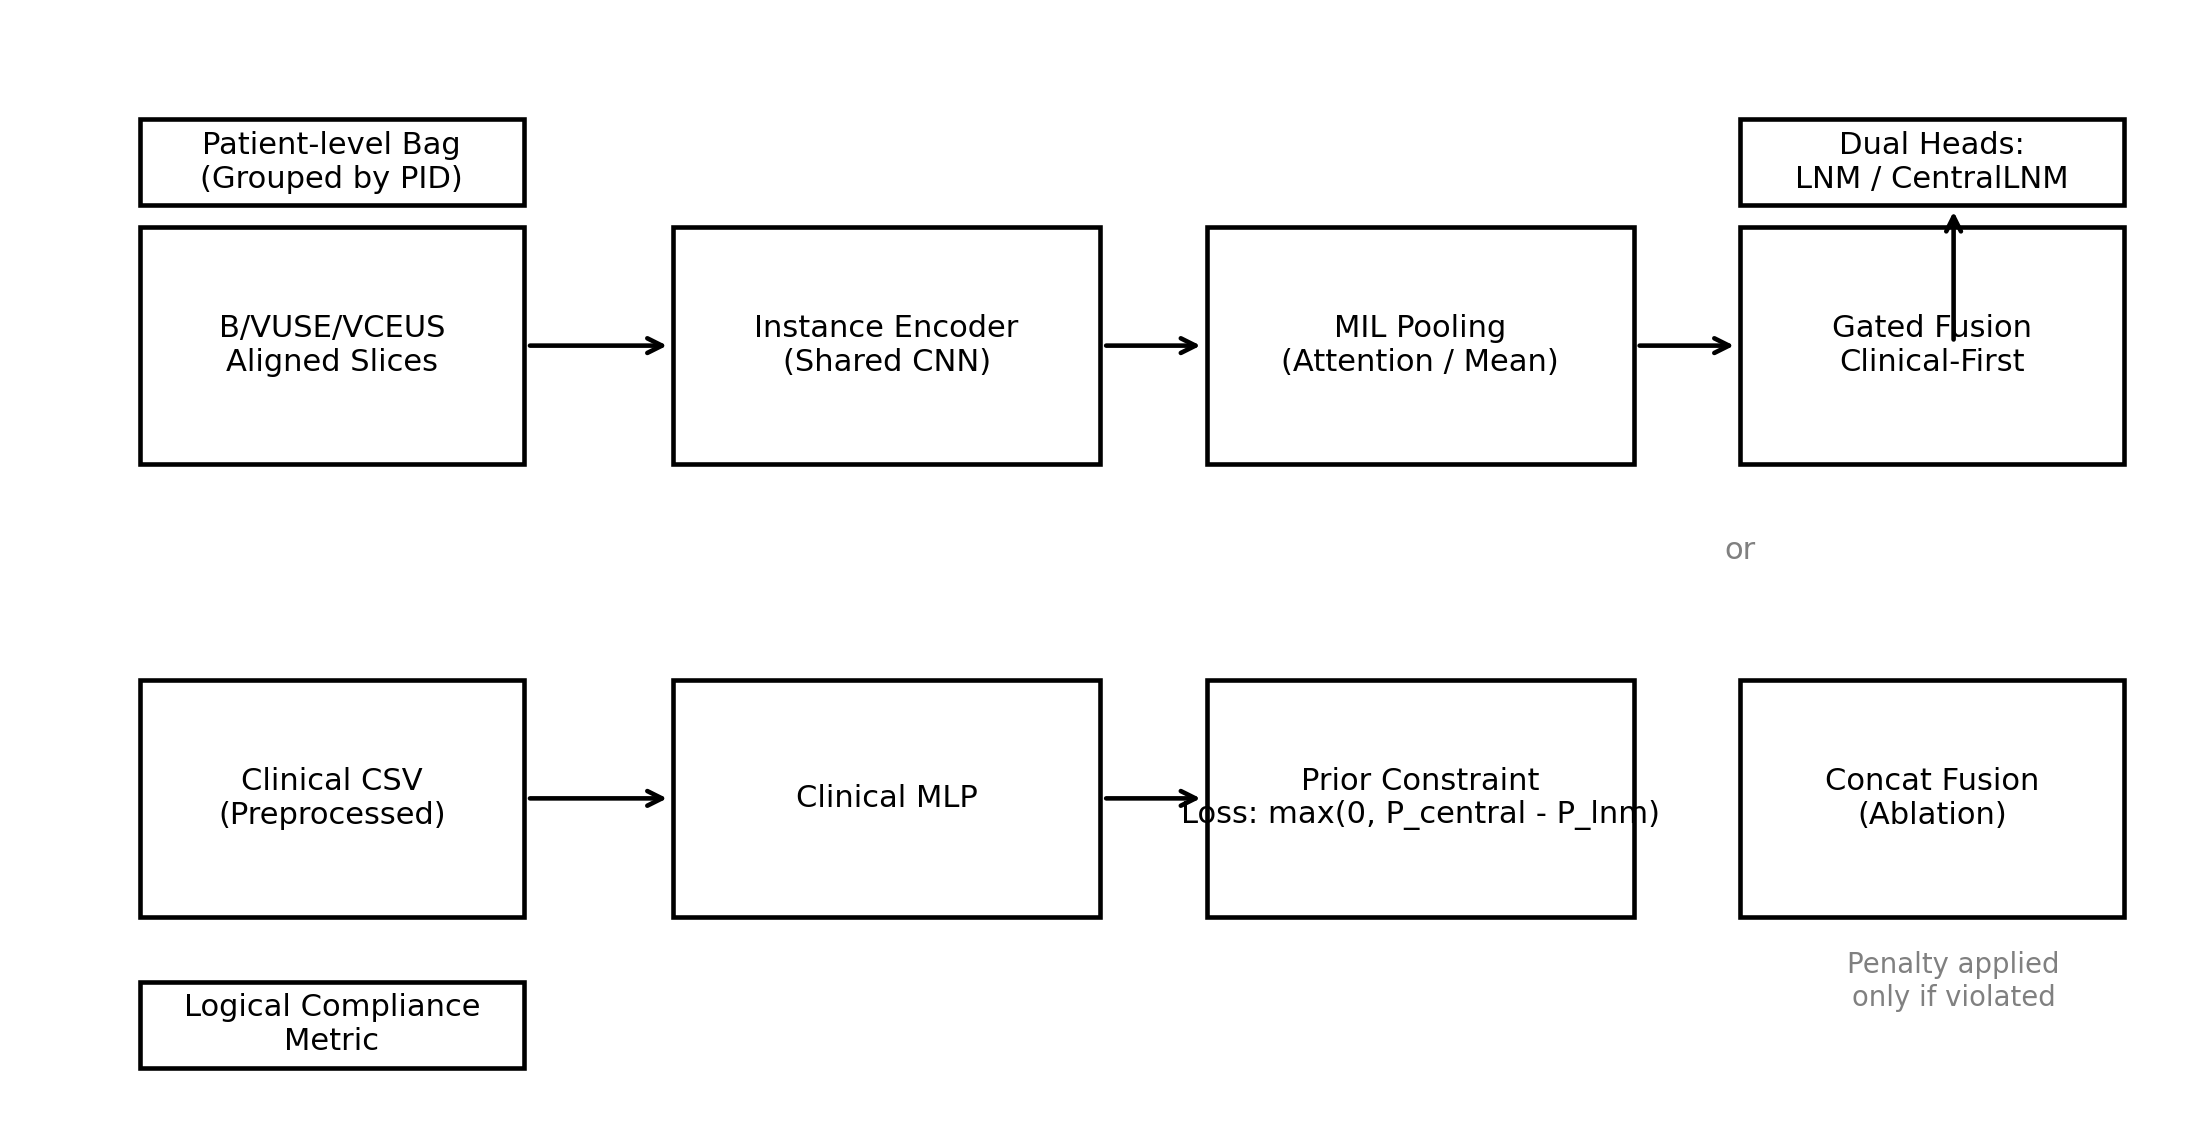
\includegraphics[width=0.92\textwidth]{figures/mil_gated_prior_arch.png}
\caption{主模型总体架构。多模态实例首先经共享编码器提取特征，再通过患者级 MIL 聚合形成影像表示；临床分支生成门控向量，对影像信息进行选择性注入，最后输出 LNM 与 CentralLNM 的联合预测。}
\label{fig:method_arch}
\end{figure}

\subsection{多架构比较、消融验证与多源融合}
在主模型框架固定后，进一步进行了三类扩展验证：
\begin{itemize}[leftmargin=1.8em]
  \item \textbf{多架构公平比较：}在统一预训练协议下比较 ResNet、EfficientNet、ConvNeXt、ViT、Swin 与 MobileViT 等骨干网络，用于评估框架对编码器选择的敏感性。
  \item \textbf{关键模块消融：}围绕 MIL 聚合方式、融合方式及先验约束进行 5 组对照（剔除 Base-A），并将 Ours 结果统一替换为 ViT-B/16 对应结果。
  \item \textbf{多源融合验证：}在深度学习与临床融合基础上引入 ROI radiomics 分支，比较 ROI Radiomics-only、Clinical+ROI Radiomics、Deep+Clinical 以及 Tri-Fusion 的表现，判断多源融合是否带来稳定受益。
\end{itemize}

\subsection{统计呈现原则}
由于本文目标是形成投稿级主文而非实验日志，结果展示遵循两条原则：一是优先保留统一协议下的核心结论，不再使用过程性排查实验主导正文；二是对复杂敏感性分析仅保留必要摘要，将逐折明细和大规模融合器网格结果转入补充材料。

此外，对于深度学习主模型，除常规定量指标外，还补充展示 ROC、校准曲线、决策曲线分析（DCA）及风险分层结果，以从判别能力、概率一致性和潜在临床净获益三个层面解释模型的临床可用性。
